%*******************************************************************************
%****************************** Second Chapter *********************************
%*******************************************************************************

\chapter{My second chapter}

\graphicspath{{Chapter2/Figs/Box1/}{Chapter2/Figs/Box2/}}



\section[Short title]{Reasonably long section title}

I'm going to randomly include a picture in Figure~\ref{fig:Figure1}.

\bigskip
\begin{figure}[htbp!]
\centering
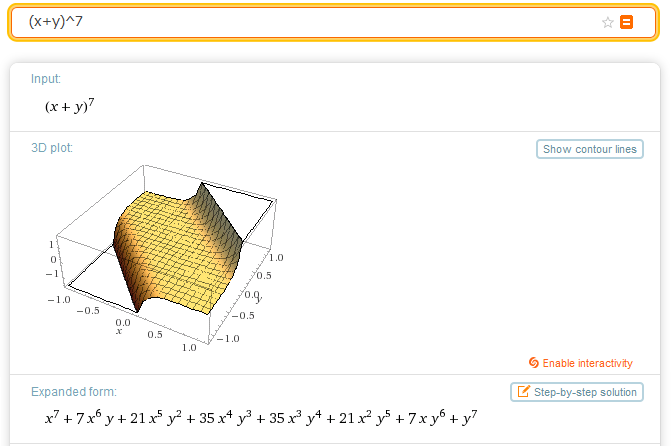
\includegraphics[width=1\textwidth]{alpha.png}
\caption[Figure 1]{This is just a long figure caption}
\label{fig:Figure1}
\end{figure}


\section*{Enumeration}
\begin{enumerate}
\item The first topic is dull
\item The second topic is duller
\begin{enumerate}
\item The first subtopic is silly
\item The second subtopic is stupid
\end{enumerate}
\item The third topic is the dullest
\end{enumerate}

\section*{itemize}
\begin{itemize}
\item The first topic is dull
\item The second topic is duller
\begin{itemize}
\item The first subtopic is silly
\item The second subtopic is stupid
\end{itemize}
\item The third topic is the dullest
\end{itemize}

\section*{description}
\begin{description}
\item[The first topic] is dull
\item[The second topic] is duller
\begin{description}
\item[The first subtopic] is silly
\item[The second subtopic] is stupid
\end{description}
\item[The third topic] is the dullest
\end{description}

\section{Second section}
Galois was born on 25 October 1811 to Nicolas-Gabriel Galois and Ad\'{e}la\"{\i}de-Marie (born Demante). His father was a Republican and was head of Bourg-la-Reine's liberal party. He became mayor of the village after Louis XVIII returned to the throne in 1814. His mother, the daughter of a jurist, was a fluent reader of Latin and classical literature and was responsible for her son's education for his first twelve years. At the age of 10, Galois was offered a place at the college of Reims, but his mother preferred to keep him at home.

In October 1823, he entered the Lyc\'{e}e Louis-le-Grand, and despite some turmoil in the school at the beginning of the term (when about a hundred students were expelled), Galois managed to perform well for the first two years, obtaining the first prize in Latin. He soon became bored with his studies and, at the age of 14, he began to take a serious interest in mathematics.

He found a copy of Adrien Marie Legendre's {\it \'{E}l\'{e}ments de G\'{e}om\'{e}trie}, which it is said that he read ``like a novel'' and mastered at the first reading. At 15, he was reading the original papers of Joseph Louis Lagrange, such as the landmark {\it R\'{e}flexions sur la r\'{e}solution alg\'{e}brique des \'{e}quations} which likely motivated his later work on equation theory, and {\it Le\c{c}ons sur le calcul des fonctions}, work intended for professional mathematicians, yet his classwork remained uninspired, and his teachers accused him of affecting ambition and originality in a negative way.\footnote{My footnote goes blah blah blah! \dots}.

While many mathematicians before Galois gave consideration to what are now known as groups, it was Galois who was the first to use the word group (in French {\it groupe}) in a sense close to the technical sense that is understood today, making him among the founders of the branch of algebra known as group theory. He developed the concept that is today known as a normal subgroup. He called the decomposition of a group into its left and right cosets a proper decomposition if the left and right cosets coincide, which is what today is known as a normal subgroup. He also introduced the concept of a finite field (also known as a Galois field in his honor), in essentially the same form as it is understood today.

In his last letter to Chevalier and attached manuscripts, the second of three, he made basic studies of linear groups over finite fields:

\begin{itemize}
    \item He constructed the general linear group over a prime field, $GL(\nu, p)$ and computed its order, in studying the Galois group of the general equation of degree $p^\nu$.
    \item He constructed the projective special linear group $PSL(2,p)$. Galois constructed them as fractional linear transforms, and observed that they were simple except if p was 2 or 3. These were the second family of finite simple groups, after the alternating groups.
    \item He noted the exceptional fact that $PSL(2,p)$ is simple and acts on $p$ points if and only if $p$ is 5, 7, or 11.
\end{itemize}


\begin{landscape}

\section*{Subplots}
I can cite AAA (see Fig.~\ref{fig:Collatz}) and BBB (Fig.~\ref{fig:Figure2}) or I can cite the whole figure as Fig.~\ref{fig:animations}


\begin{figure}
  \centering
  \begin{subfigure}[b]{0.55\textwidth}
    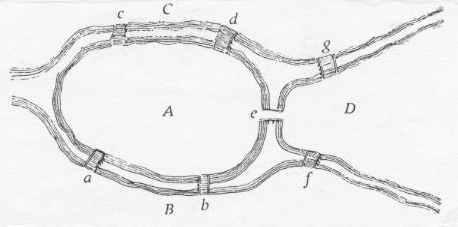
\includegraphics[width=\textwidth]{setepontes}
    \caption{7 Bridges}
    \label{fig:7 Bridges}
  \end{subfigure}
  \begin{subfigure}[b]{0.42\textwidth}
    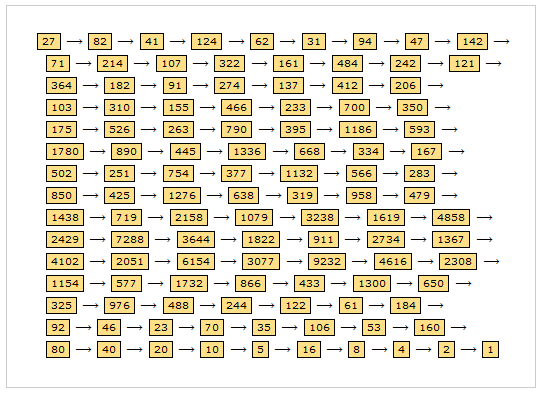
\includegraphics[width=\textwidth]{collatz}
    \caption{Collatz}
    \label{fig:Collatz}
  \end{subfigure}
  \begin{subfigure}[b]{0.42\textwidth}
    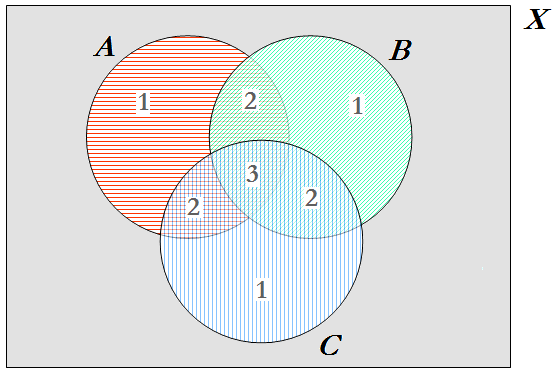
\includegraphics[width=\textwidth]{venn}
    \caption{Venn diagram}
    \label{fig:Figure2}
  \end{subfigure}
  \caption{Best Pictures}
  \label{fig:animations}
\end{figure}

\end{landscape}

\section{Third section}

\tochide\section{Hidden section}



